\chapter{Skin recognition}
    Earlier, we have described why liveness detection is an important part
    of a face recognition system and why it could greatly improve security.
    We focused on using light reflectiveness to recognize skin on photos.
    This idea comes from the fact that every material has its own, unique spectrum.
    Different types of human skin reflect visible light very differently,
    but those differences become smaller when going further into infrared wavelengths
    \cite{visinfra} \cite{toyotaskin}, which is why we decided to use infrared light
    in our experiments.

    Additionally, with the information of which pixel contains human skin,
    it would be possible to use this to remove the background from face photos.
    As described in a later chapter, this is an important part of face recognition,
    and is currently done using methods based on machine learning, which are usually
    rather slow.
    Using skin detection could significantly improve the performance of background
    removal.

    \section{Technical aspect -- how does a camera work?}
        To think about security aspect of skin detection,
        it's critical to understand how image sensors works.
        The most common sensors are \textit{CCD} (\textit{charge-coupled device})
        and \textit{CMOS} (\textit{complementary metal-oxide-semiconductor})
        [TODO: LINK NEEDED].
        Due to better quality, as well as sensitiveness, for security reasons
        it probably would be better to use CCD.
        However, both matrices have same problem -- limitation on wavelength sensitivity.
        Such sensors are sensitive to wavelengths approximately up to 1050nm,
        which may be a serious limitation as human skin has more undifferentiated
        characteristics in greater wavelengths.
        Therefore looking for the the best possible skin detection method,
        it may be convenient to assume that other type of light sensitive matrices
        are in reach of inventor.
        Nevertheless we were limited to very common cameras.

        TODO: Paragraph about light sensors materials and other types of image sensors.
        Paragraph under maintenance. May disappear.

        We are describing one possible realization, keep in mind that
        there are more solutions than that, but we do not find them
        useful in our problem.

        \subsection*{Monochrome}
            As image sensor is matrix build from many small photodiodes,
            it's natural to create monochromatic image.
            Because photodiodes don't distinguish different
            wavelength, only light intensity, it's hard
            to measure light reflectiveness.
            The only possible way to do that is to
            make different picture for every wavelength.
            It's not easy, as you have to
            provide your own lighting and somehow remove
            light coming from other sources.
            Also, all pictures have to be made in
            a~very short time interval, as the subject
            cannot move between shots.

        \subsection*{Multispectral imaging}
            Multispectral imaging is an answer to the problem of the object moving,
            it is a way to measure every wavelength intensity in one picture.
            Probably the easiest way to describe it is to look at RGB camera.
            There, every photodiode is responsible for exactly one color,
            where as color we understand wavelength interval (it's important
            to understand, that we can consider any wavelength interval as one color).
            And result picture is built from small squares (mostly $2 \times 2$)
            of photodiode matrix data.
            There may be more than just three colors in fact.
            For example, you may find a camera which can see two types of ''green''.
            Mostly, at the end everything is converted to known RGB format.

            \begin{figure}[H]
                \caption{RGB image sensor matrix with two types of green -- sensors assignation.}
                \centering
                \includegraphics{RGB-matrix}
                \label{fig:RGB-matrix}
            \end{figure}

            Software receives from camera information with light intensity at every
            sensor and information which color it sees.

            One of possible realizations of reducing the range
            of light visible through the sensor is to take standard image sensor which
            may see full spectrum of light ($350$-$1050$nm.) and place filters
            in the way that only specific light will reach the chosen photodiode.

            \begin{figure}[H]
                \caption{Visualization of how filters works.}
                \centering
                \includegraphics[scale=0.40]{RGB-filter}
                \label{fig:RGB-filter}
            \end{figure}

        \subsection*{Hyperspectral imaging}
            Hyperspectral imaging is creating pictures using a camera with the
            capability to distinguish many colors
            (even hundreds or thousands) instead of just few.
            It would be very helpful, obviously, in skin-detection device,
            but there is very little chance to see such device in mobile phones soon.

    \section{Technical aspect -- how it may be created?}
        As we know how camera works, we can say that there are only two ways of
        building skin detection mobile device.
        \subsection*{Monochrome}
            We can work without filters (or with one for whole camera),
            but then we have to make picture for every wave length.
            Also, we need one diode with that very wavelength we want.
            It's easier method to build in phone, but taking pictures
            must be very fast.

            Biggest pros of that solution is possibility of lighting
            with different LEDs in random moment of time, so hackers
            will no be able to play with own diodes to modify result.

        \subsection*{Multispectral imaging}
            Also there is possibility to use filters with specific infrared colors.
            But important here is avoiding standard smoothing algorithms used
            in cameras. We truly need real light intensity from every sensor.
            Not smoothed or reduced one.

    \section{Our attempts}

        \subsection{Detecting reflectiveness using Kinect}
            Our first idea was to use a Kinect v2 depth and infrared camera to detect
            how well does a surface reflect light.
            Kinect v2 cameras have their own source of infrared light and they make
            a very good job at filtering other sources of light.
            So, for each pixel on the infrared image, we know how much light coming
            from the Kinect's light emitter was reflected in that particular place.
            Also, Kinects are depth cameras, which additionally gives us the information
            on how far away from the camera is the object visible on that pixel.

            Since the source of light is in the same device as the camera, the distance
            seen on the depth image is also the distance from the light emitter.
            This is an important observation, because we know how distance affects how
            much light arrives at a particular place. % might need a better wording
            If we have a source of light that, at a given distance, lights up a
            1cm $\times$ 1cm square of a flat surface with a particular amount
            of light, then at double that distance it will light up a 2cm $\times$ 2cm
            square with the same amount of light, which means that the same amount
            of light is distributed over a 4 times larger surface, so the
            intensity of light has to be 4 times lower than before.

            With those observations, we took pairs of IR and depth images, and for each
            pixel calculated a new value of $ir\_intensity \cdot depth \cdot depth$,
            which should estimate how well light was reflected at that point,
            regardless of distance from the camera.

            \begin{figure}[H]
                \caption{An unprocessed IR photo, and an image calculated using
                the method described above.}
                \centering
                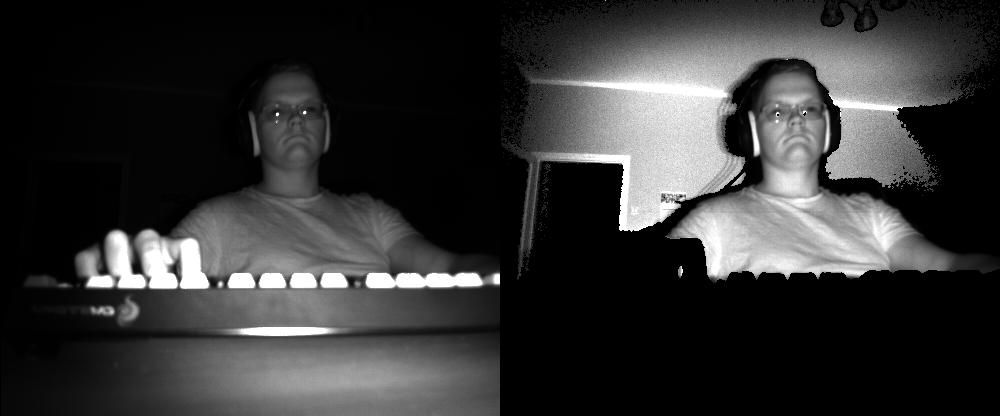
\includegraphics[width=\textwidth]{skin_kinect_1}
                \label{fig:skin_kinect_1}
            \end{figure}

            As seen on figure \ref{fig:skin_kinect_1}, we have accidentally created
            a night vision camera (please note that some of the black areas are there because Kinect cameras do not give depth data for objects closer than 50cm)
            -- but this means that our idea is to some extent working, because the point
            of it was to make objects in the distance indistinguishable from those close
            to the camera.

            However, one this that is not considered in that method is that objects
            can also be at different angles to the camera.
            A sheet of paper perpendicular to the source of light will reflect more
            light to the Kinect than it would reflect if it was at a 45 degrees angle.

            \begin{figure}[H]
                \caption{Three IR images processed with the described method, with a
                manually determined interval of values marked red.}
                \centering
                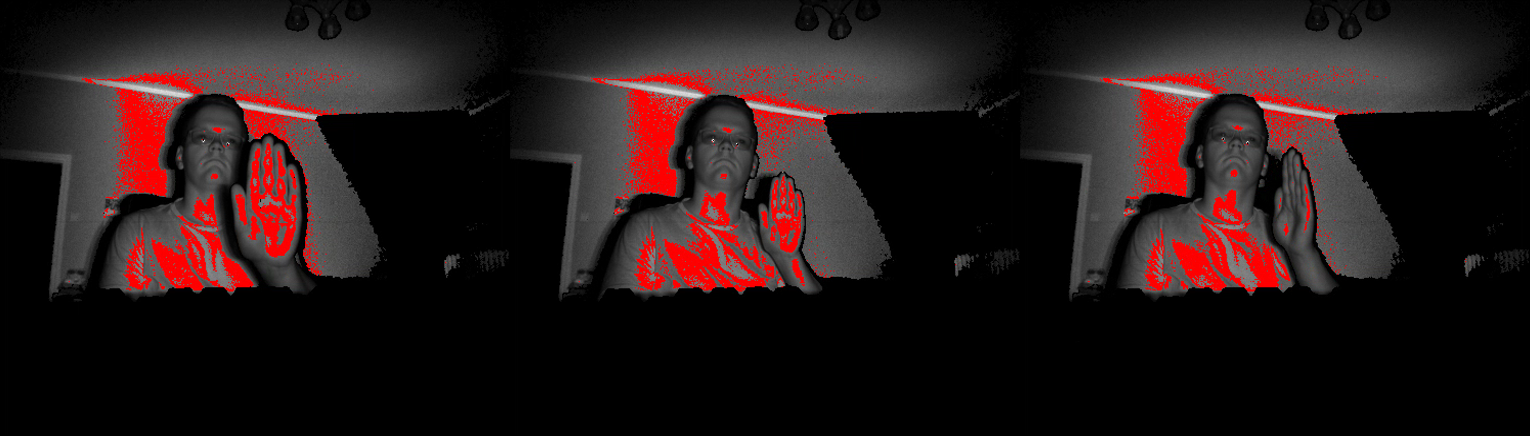
\includegraphics[width=\textwidth]{skin_kinect_2}
                \label{fig:skin_kinect_2}
            \end{figure}

            We have manually selected an interval of values and marked them red, which
            can be seen on figure \ref{fig:skin_kinect_2}.
            On the first two pictures there, the hand is at the same angle, but at a
            different distance to the camera.
            It is visible that the calculated values remained very close regardless
            of the distance, which was a success.
            However, on the third picture, the hand is at a different angle and
            that changes how it reflects light towards the camera, which makes the values
            different.

            Knowing the depth value and certain properties of the camera, it is possible
            to calculate the 3D coordinates of each pixel.
            With that information, it is possible to calculate the angle towards the
            camera between each two pixels, and then use that value in the method above
            to make it independent of angles.
            However, our attempts to do this were unsuccessful, possibly because the
            depth camera is not precise enough.
            % TODO Dominik: maybe describe briefly the mathematical details of what
            %               was attempted

        \subsection{Using three infrared wavelengths}
            \subsubsection*{Prototype}
            With the previous method using only one light wavelength (the one emitted by
            Kinect), we decided to take photos using three different wavelengths.
            This gives the opportunity to analyze how does the way the objects reflect
            light changes with regard to light wavelength, instead of directly looking
            at how bright a point is.

            To make any research, we had to take three photos of the same object
            reflecting three different wavelengths of infrared light.
            The camera, the infrared light sources, and the photographed object
            had to be in the same position for all of the photos.
            An ideal way to do this would be to use a multispectral camera, but they are
            very expensive and we were not able to use one.

            One possible way to take a photo of how a certain wavelength is reflected
            would be to use a filter that only lets that wavelength to pass through it.
            However, changing filters on the camera between taking photos would take
            a lot of time, which would create a risk of changing the relative position
            of the object and the camera, which is unacceptable.

            We borrowed a mobile phone which had a filter mounted on its front camera
            that allowed various wavelengths of infrared light, but not visible light.
            This opened up the opportunity to take a different approach -- instead
            of filtering the selected wavelength, we want to illuminate the object
            using only that wavelength.

            We purchased diodes emitting light in the following wavelengths:
            850nm, 890nm, 940nm. Those diodes were connected to an Arduino board.
            We used two diodes of each wavelength, and mixed their positions to
            make sure that the centers of sources of light at each wavelength
            are as close as possible.

            \begin{figure}[H]
                \caption{Arduino board with six IR diodes.}
                \centering
                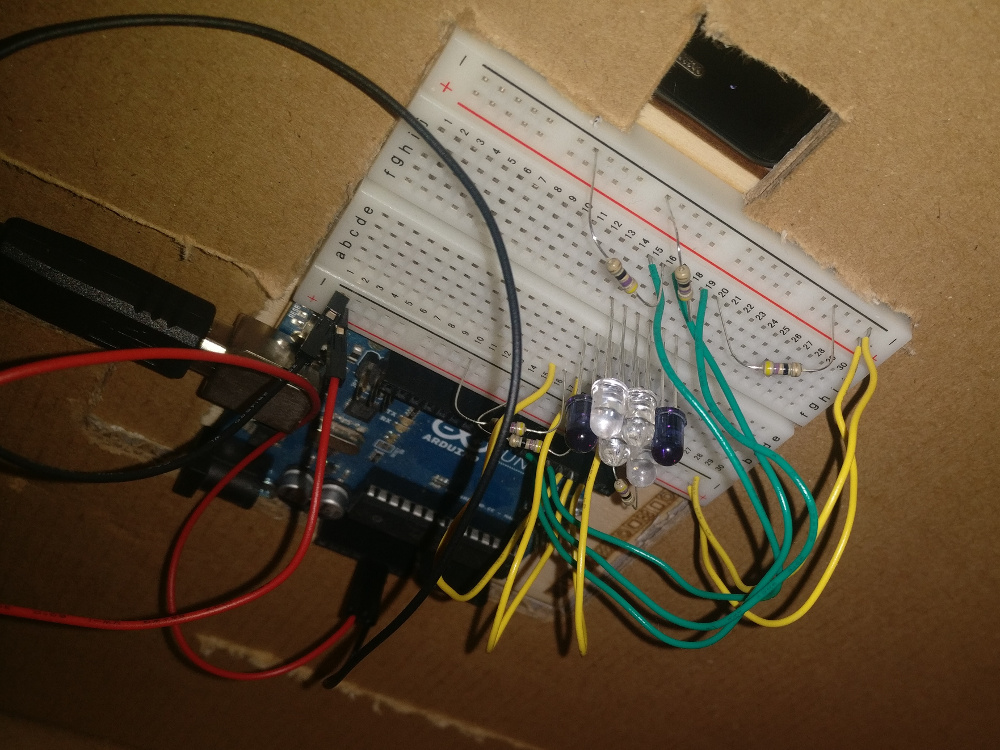
\includegraphics[height=7cm]{arduino_1}
                \label{fig:arduino_1}
            \end{figure}

            Since taking all three photos at the same time would be impossible,
            we stabilized the camera and the diodes by putting them in holes
            in a cardboard box.

            \begin{figure}[H]
                \caption{Outside view of the Arduino board and the camera.}
                \centering
                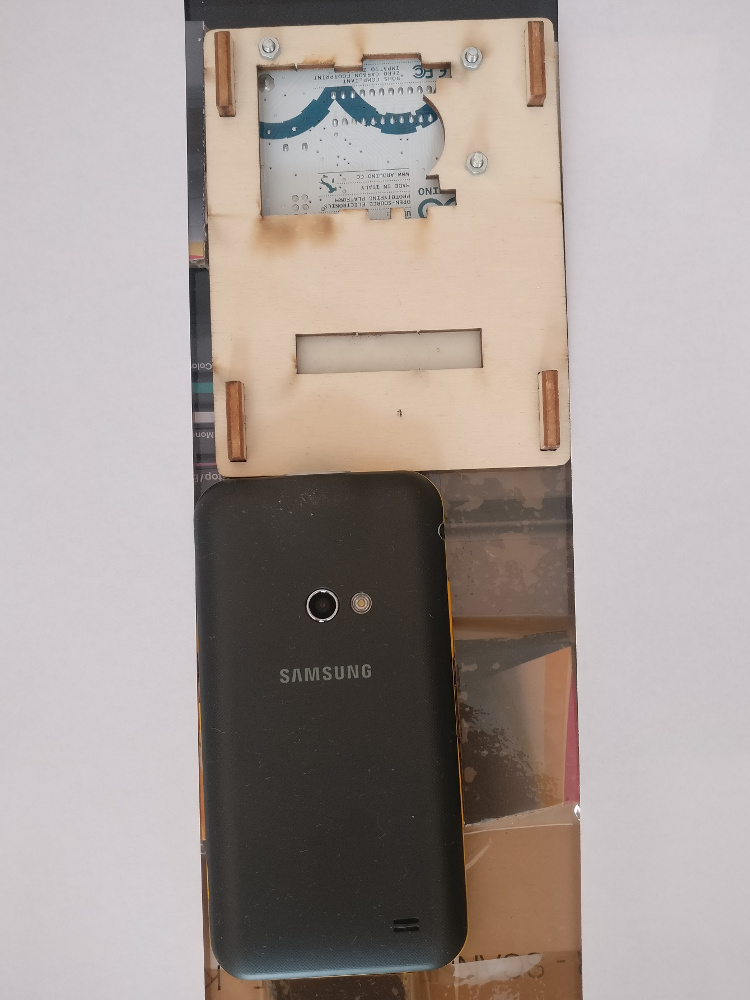
\includegraphics[height=7cm]{arduino_2}
                \label{fig:arduino_2}
            \end{figure}

            With this setup, all that remained to do was to take more photos.
            The camera and the phone were stable, but when photographing for example
            a human hand, it might move.
            The photos have to be taken in the smallest possible intervals
            and human interaction can not be required while taking them,
            because that could result in moving the camera or the diodes.

            Turning specific diodes on and off was a rather easy task.
            Arduino is by definition programmable, so we just wrote a program that
            listened to data sent on a USB cable and turned on the requested diode.\\
            We found an Android app \cite{opencameraremote} designed to take photos
            remotely when commanded so from another phone with a special pilot app.
            It is open source, so we read its source and found out that it just sends
            simple broadcast messages through LAN.

            With this information, we were able to write a Python script that did the
            following:

            \begin{itemize}
                \item connect to Arduino through USB, turn on 850nm diodes
                \item wait 0.75 seconds
                \item send a broadcast message to take a photo
                \item wait 0.75 seconds
                \item turn on 890nm diodes
                \item wait 0.75 seconds
                \item take a photo
                \item ... -- analogical procedure to take a photo with 940nm light
            \end{itemize}

            Since we were using only the front camera from a relatively old phone,
            we had to take a 1.5 seconds break between each photo -- otherwise
            there was a significant chance of the camera app not catching one of the
            broadcasted commands and taking only two photos.
            The time between the first and last of three photos was 3 seconds,
            and that was an acceptable delay to make sure that the photographed
            object was in a stable position.

            \begin{figure}[H]
                \caption{Photos taken with 850nm, 890nm, and 940nm light respectively.}
                \centering
                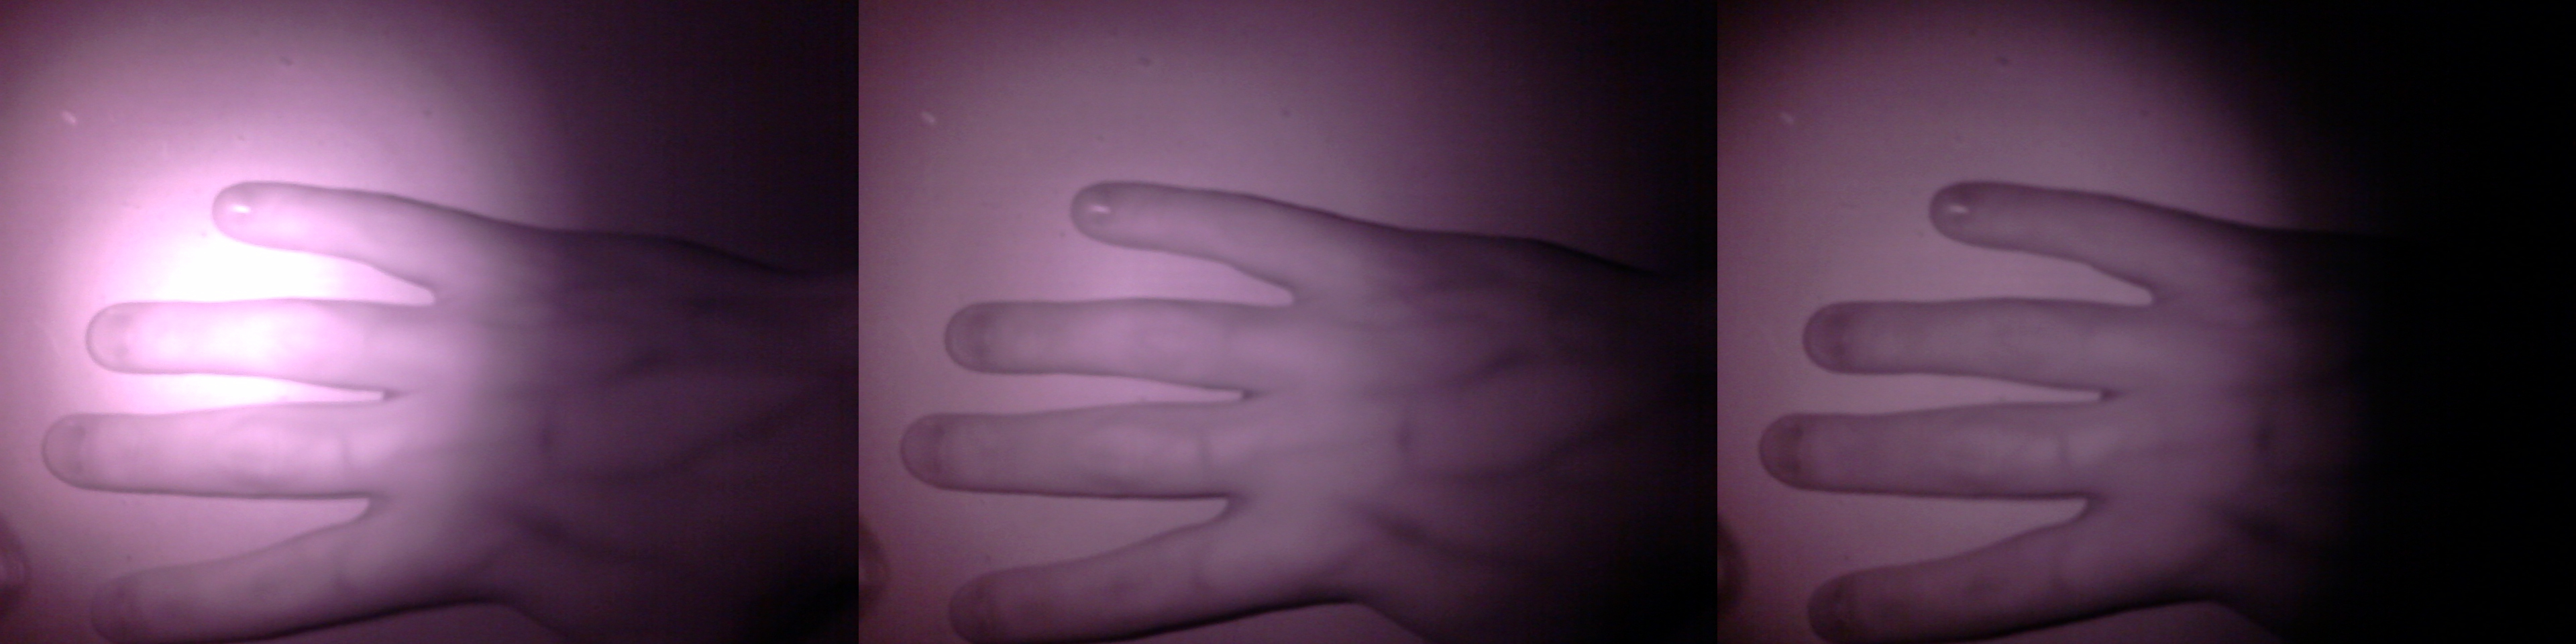
\includegraphics[width=\textwidth]{ir_photos}
                \label{fig:ir_photos}
            \end{figure}

            \subsubsection*{Detecting skin -- preprocessing}
                As we had phone's camera (with not fully known filter)
                our input was picture-matrix
                in which every pixel was nine elements tuple.
                In fact values there wasn't independent, because
                in every taken JPG occurred $R \approx B \approx 2 \cdot G$
                for almost every pixel.
                Therefore using all that data was helpful only to overfit,
                not to improve model.

                We had many preprocessing ideas, but all were focused
                on using every pixel independently.
                The one with best results (in fact only slightly better,
                but not negligibly) was taking one value from every
                of three pictures and calculating ratios.
                There is chance to improve preprocessing using more than one pixel,
                but we were focused on problem with more reliable results.

            \subsubsection*{Detecting skin -- models}
                Unfortunately, handmade algorithm to detect skin failed,
                so we decided to use machine learning.
                We prepared image masks to hand picture,
                so it was easy to provide information to algorithm, which
                pixel is skin pixel, and which is not.

                [TODO: MASK PIC]

                We have used scikit-learn to test different models.
                We had hope that SVM will work correctly,
                and in fact with linear kernel it worked very well.
                However, Random Forest had slightly better results.

                [TODO: SVM PIC]

                \begin{figure}[H]
                    \caption{TODO: BETTER PIC FOR RANDOM FOREST}
                    \centering
                    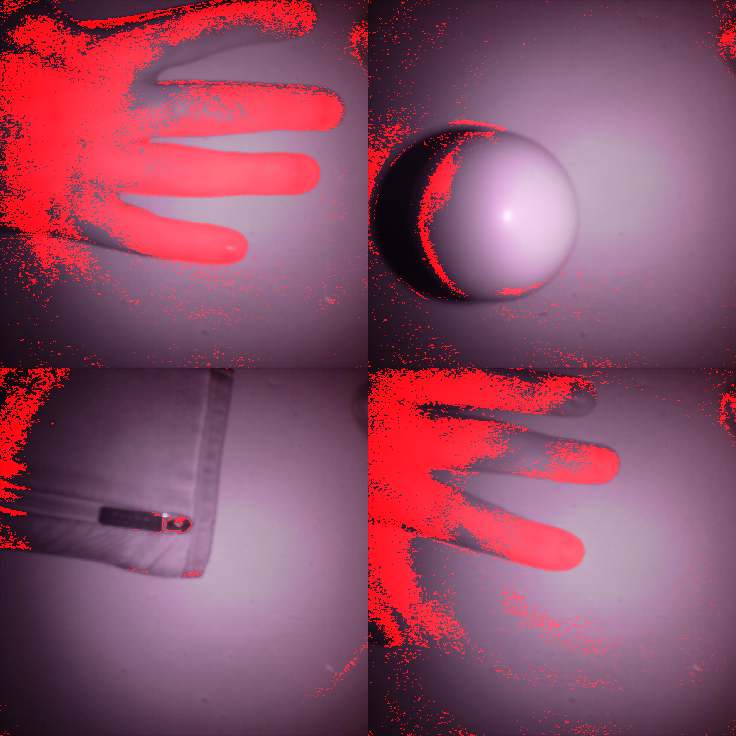
\includegraphics[width=10cm]{skin_results}
                    \label{fig:skin_results}
                \end{figure}

                It's important to notice that we had pictures
                with big part of information lost,
                as we wasn't able to take RAW photo or at least
                avoid JPEG compression. It was visible very good
                when we tried to overfit on some images, and
                we failed. There were no enough information event to overfit.
                Therefore we consider our results as better than expected.

                [TODO: RANDOM FOREST OVERFITTING PIC]

    \section{Results}
        The results achieved by our skin detection were far from perfect,
        however we still think that using infrared photos to analyze surface
        reflectiveness and using that to detect skin is a promising method.
        We were very limited by the low quality and JPEG compressed photos,
        overall lack of high quality hardware, and our lack of knowledge in electronics,
        but were still able to achieve results that visually make sense.
        With more resources, we believe this could increase security of
        face authentication solutions.

    \section{RGB skin detection simulation}
        Because we wanted to have the ability to check how skin detection
        (if it was implemented in a possible future device) could be utilized
        by other algorithms, but we couldn't integrate our prototype with
        anything else, we prepared a skin-detection heuristic based on RGB images.
        We based our algorithm on transformation from
        \citation{toyotaskin}:
        \[
            \begin{bmatrix}
                Y \\
                Cb \\
                Cr
            \end{bmatrix}
            =
            \begin{bmatrix}
                16\\
                128\\
                128
            \end{bmatrix}
            +
             \begin{bmatrix}
                 0.257  &  0.504        &  0.098 \\
                -0.148  & -0.291        &  0.439 \\
                 0.439  & -0.368        & -0.071
            \end{bmatrix}
            \cdot
             \begin{bmatrix}
                R\\
                G\\
                B
            \end{bmatrix}
        \]

        However, conditions described in paper gave us too many false positives (what is understandable),
        so we decided to improve decision process. If we will name vector $(Y, Cb, Cr)$ for pixel $p = (R, G, B)$
        mark of $p$, then we calculated for every pixel in image it's mark.
        After that we were taking a few marks of pixels from central part of image and
        sorting them by euclidean norm.
        Heuristically middle element of new table is skin picture.
        At the end, we consider every pixel as skin pixel if and only if
        it's mark was close enough to middle mark from sorted list.

        \begin{figure}[H]
            \caption{RGB skin detection heuristic.}
            \centering
            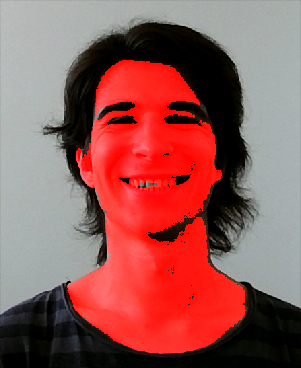
\includegraphics[scale=0.7]{skin_detection_heuristic}
            \label{fig:skin_detection_heuristic}
        \end{figure}
